\documentclass[conference]{IEEEtran}
\IEEEoverridecommandlockouts % Required for funding footnotes
% The preceding line is only needed to identify funding in the first footnote. If that is unneeded, please comment it out.
% \usepackage{cite}
\usepackage{hyperref}
\usepackage{amsmath,amssymb,amsfonts}
\usepackage{algorithmic}
\usepackage{graphicx}
\usepackage{textcomp}
\usepackage{xcolor}

\def\BibTeX{{\rm B\kern-.05em{\sc i\kern-.025em b}\kern-.08em
    T\kern-.1667em\lower.7ex\hbox{E}\kern-.125emX}}
\begin{document}

\title{An Explainable Multimodal Neural Framework for Financial Risk Management\\
% {\footnotesize \textsuperscript{*}Note: Sub-titles are not captured in Xplore and
% should not be used}
% \thanks{Identify applicable funding agency here. If none, delete this.}
}

\author{
\IEEEauthorblockN{Ibrahim Hussain}
\IEEEauthorblockA{\textit{Department of AI \& Data Science} \\
\textit{FAST NUCES}\\
Islamabad, Pakistan \\
ibrahimbeaconarion@gmail.com}
\and
\IEEEauthorblockN{Lubabah Moten}
\IEEEauthorblockB{\textit{Department of AI \& Data Science} \\
\textit{FAST NUCES}\\
Islamabad, Pakistan \\
lubabahmoten@gmail.com}
\and
\IEEEauthorblockN{Sabeel Nadeem}
\IEEEauthorblockC{\textit{Department of AI \& Data Science} \\
\textit{FAST NUCES}\\
Islamabad, Pakistan \\
sabeelnadeem15@gmail.com}
}

\maketitle

% \section*{\textbf{ABSTRACT}}
% \begin{abstract}
%  Financial markets are noisy and unpredictable, yet most AI models operate as black boxes that cannot explain their decisions. This lack of transparency makes them unreliable for financial risk management. This paper proposes an explainable distributed deep learning framework that breaks financial risk management into specialised modules. The system presents five data modalities: market time series, SEC text filing, macro indicators, company fundamentals and cross-asset graph structures. A temporal attention encoder learns from market sequences while three analysts(technical, sentiment and news)process different signals. These feed into a risk engine that combines volatility, drawdown, VaR, CVaR, contagion, liquidity and regime detection modules. A position sizing engine determines exposure, and an xAI layer provides explanations for every decision. The framework achieves strong performance as the news analyst achieves strong F1 scores with perfect recall. The liquidity module shows high tradability across the asset universe, and the VaR rate falls closer to the expected threshold. The system outputs Buy/Hold/Sell decisions with confidence scores, position sizes, risk summaries and human-readable explanations. Our work is accessible at \textmd{\texttt{\url{https://github.com/ib-hussain/fin-glassbox}}}.
% % Explainable AI, Financial Risk Management, Deep Learning, FinBERT, Graph Neural Networks, Risk Engine, Multimodal Learning, Neural Framework.
% % }
% \end{abstract}
\begin{abstract}
Financial markets are noisy and unpredictable, yet most AI models operate as black boxes that cannot explain their decisions. This lack of transparency makes them unreliable for financial risk management. This paper proposes an explainable multimodal neural framework that breaks financial risk management into specialised modules. The final system uses four active data streams: market time series, SEC text filings, FRED macro/regime indicators and cross-asset graph structures. A temporal attention encoder captures relationships from market sequences, while FinBERT encodes financial text. These signals feed into a risk engine that combines volatility, drawdown, VaR, CVaR, StemGNN-based contagion risk, liquidity risk and MTGNN-based regime detection. The regime module combines temporal embeddings, FinBERT text embeddings, learned graph properties, and FRED macro features to classify market state. A position sizing engine determines exposure, and an xAI layer provides explanations for every decision. Results show that the framework produces risk-aware Buy/Hold/Sell decisions with confidence scores, position sizes, risk summaries and human-readable explanations. Our work is accessible at \textmd{\texttt{\url{https://github.com/ib-hussain/fin-glassbox}}}.
\end{abstract}


\section{Introduction}

Financial markets are noisy, high-risk and constantly changing. Although modern AI models can produce accurate predictions, many of them operate as black boxes, which makes them difficult to trust in financial decision-making. In this domain, a correct prediction is not enough. A user must also understand why a trade was suggested, what risks were considered and why a certain position size was chosen.

Recent work shows that graph neural networks can capture complex relationships between financial assets, while xAI research highlights the need for interpretable and explainable financial forecasting systems \cite{financesurvey,12thPaper}. Uygun and Sefer \cite{13thPaper} showed that graph-based temporal models such as MTGNN and StemGNN can handle complex financial time-series patterns better than older sequential methods. Similarly, TradingAgents demonstrates the value of dividing financial reasoning among specialised agents, but its LLM-based structure is harder to reproduce and does not directly provide trained numerical risk modelling \cite{1stPaper}.

These works show that financial AI benefits from graph modelling, specialised components and explainability. However, existing systems usually focus on prediction, agent reasoning or post-hoc explanations separately. They rarely combine multimodal encoders, classical risk measures, graph-based contagion, regime detection, position sizing and xAI into one auditable framework. This gap motivates our proposed architecture.

\section{Problem Statement}

This work addresses the problem of producing risk-aware and explainable financial decisions from multimodal market data. The system uses four active data streams: market time-series data, SEC text filings, macro/regime indicators and cross-asset graph structures. Given these inputs, the framework produces a Buy/Hold/Sell decision, confidence score, position size, risk summary and explanation trace. The objective is not only to improve prediction, but to make every decision inspectable. The user should be able to see which signals supported the decision, which risks reduced exposure and whether any rule-based safety barrier changed the final output. In this sense, the goal is to turn a black-box financial model into a glass-box decision system.

\section{Dataset Preparation}

The framework uses four active data families: SEC textual filings, macro/regime indicators, market time-series data and cross-asset relation graphs. Company fundamentals were collected during early data engineering, but were removed from the final modelling pipeline because their overlap with the final market universe was limited.

SEC textual data was collected from EDGAR filings, including 10-K, 10-Q, 8-K and DEF-14A documents \cite{SECedgarSite}. A CIK-to-ticker filtering step identified 5,644 publicly traded U.S. companies as the initial filing universe. The text pipeline performed inventory construction, cleaning, section extraction, quality checks, balancing and chunk generation for FinBERT encoding. Around 288k raw filings were collected. Since some years had weak coverage, targeted top-ups were used to improve chronological balance without duplicating existing filings.

Macro/regime data was collected from FRED to represent wider economic conditions such as interest rates, inflation-related variables, credit spreads, recession indicators and other stress markers \cite{fredSite}. More than 11,000 available series were filtered down to 49 interpretable features with sufficient 2000--2024 coverage. Since macro series have different reporting frequencies, they were aligned to trading days using leakage-aware forward filling.

Market data formed the main input for the temporal encoder, technical features, risk engine, liquidity module and graph construction. The initial market panel had incomplete coverage, so data from Yahoo Finance, Stooq, the Huge Stock Market Dataset and a Kaggle NYSE/NASDAQ dataset were merged \cite{yahooFinance,stooq,hugeMarket,nyseKaggle}. Price-scale differences were handled using overlapping-date adjustment ratios. The final universe was reduced to the 2,500 tickers with strongest coverage, and remaining gaps were filled using interpolation, ARIMA-style reconstruction and sector-based KNN imputation, followed by distribution checks.

The cross-asset relation graph was derived from the final market panel. It used rolling return correlations, SIC-code sector mapping, ETF return similarity, median dollar volume as a market-cap proxy and beta versus SPY. The final graph dataset contained 313 rolling correlation snapshots, 8,578 static edges, 2,515 graph nodes and a sample NetworkX graph with 105,545 edges. These graph outputs support the StemGNN contagion module and the MTGNN-style regime module.

\section{Proposed Framework}
The proposed framework is a neural system. The entire system can be divided into 3 layers. The system works on 512-dimensional embeddings as inputs. %Each module is supposed to take its inputs from its upstream module(s), perform the train/test/val on it and convey its outputs to its downstream modules.

\subsection{Encoder Layer}

\subsubsection{Temporal Market Encoder}
The Temporal Market Encoder converts recent market behaviour into a continuous embedding that can be reused by downstream modules. It processes 30-day market windows and uses an attention-based architecture trained from scratch through self-supervised masked reconstruction. This allows the encoder to learn return dynamics, volume-price behaviour and cross-feature interactions without requiring direct trading labels at this stage.

Feature normalisation is fitted only on the training split of each chronological chunk. The same training-fitted normaliser is then reused for validation and test data to prevent look-ahead bias. The output embedding is therefore a train-safe market representation. Its attention outputs can also be inspected, but they are treated as representation-level explanations rather than final decision explanations.

\subsubsection{Financial Text Encoder}
The Financial Text Encoder uses FinBERT because SEC filings contain domain-specific financial language, including accounting terms, risk disclosures, management discussion and forward-looking statements \cite{FinBERT}. FinBERT is adapted to our SEC corpus using masked language modelling, so this stage improves financial text representation but does not directly learn returns, sentiment labels or risk classes. Those tasks are handled later by the Sentiment and News Analysts.

After domain-adaptive training, 768-dimensional mean-pooled FinBERT embeddings are extracted from the frozen model. These embeddings are then reduced to 256 dimensions using IncrementalPCA \cite{IncrementalPCA}. The PCA projection is fitted only on training embeddings and then applied to validation and test embeddings. %This keeps the text stream consistent with the no-leakage design used throughout the framework.
\begin{figure}[t]
    \centering
    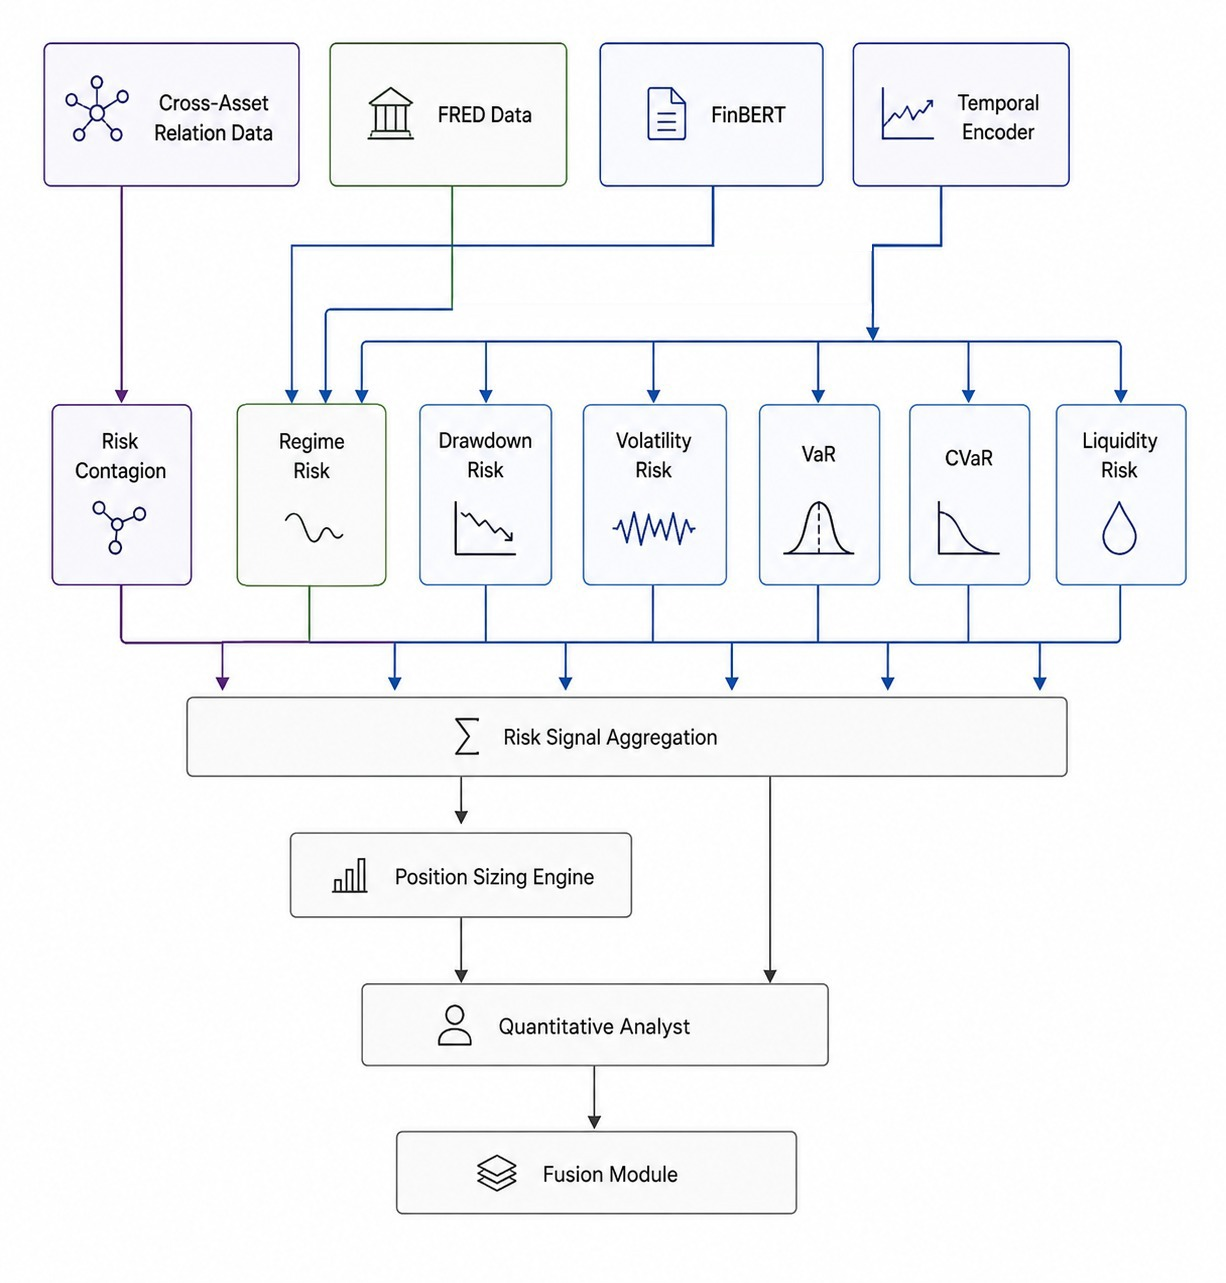
\includegraphics[width=\columnwidth]{conference-paperFigure.png}
    \caption{Proposed framework workflow showing the data streams in the encoder layer, risk modules, and the synthesis layer.}
    \label{fig:workflow}
\end{figure}
\subsection{Risk Engine}
% \subsubsection{Contagion Risk Module}
% The Contagion Risk Module answers the question
% \begin{quote}
% If market stress propagates through related assets, how vulnerable is each stock over 5, 20, and 60 trading days?
% \end{quote}
% It uses a StemGNN\cite{StemGNN} to learn how financial distress propagates through the market. For each of the 2,500 stocks, it outputs a contagion probability score (0-1) at three horizons: 5 days, 20 days, and 60 days. StemGNN is appropriate for contagion risk because it learns both graph structure and temporal structure. It is stronger than a simple correlation matrix because contagion can be non-linear, lagged, multi-hop, and regime-dependent. A StemGNN includes:
% \begin{itemize}
%     \item a latent correlation layer;
%     \item graph Fourier transform operations;
%     \item spectral-temporal processing;
%     \item multi-hop propagation through a learned adjacency matrix;
%     \item residual/stacked temporal modelling;
%     \item learned node-level outputs for all stocks simultaneously.
% \end{itemize}
% In this project, StemGNN is adapted from a forecasting model into a risk-classification model.
% StemGNN was chosen over simpler approaches (correlation matrices, linear models) because it solves:
% \begin{itemize}
%     \item non-linear contagion, crash propagation is non-linear, and StemGNN's spectral convolutions capture this
%     \item Hidden relationships, the latent correlation layer learns connections that simple correlation misses
%     \item Temporal dynamics, contagion changes over time, and Fourier transforms capture cyclical patterns
%     \item Joint learning, learns graph structure and temporal patterns simultaneously, not separately. 
% \end{itemize}
% For hyperparameter search, we run 50 trials per chunk, and 10 epochs per trial. For full training, we run 100 epochs per chunk with an early stopping patience of 20 epochs and a dropout rate of 0.75.
\subsubsection{Contagion Risk Module}
The Contagion Risk Module predicts how stress can spread from one asset to another. Financial assets do not move independently. If one stock falls sharply, related stocks in the same sector, ETF group or correlation cluster may also become vulnerable. This module, therefore, answers the question:
\begin{quote}
If market stress propagates through related assets, how vulnerable is each stock over 5, 20 and 60 trading days?
\end{quote}

For this module, we use StemGNN\cite{StemGNN} because contagion is naturally a graph problem. The input is the cross-asset relation graph built from market-derived relationships such as rolling correlations, sector links, beta estimates and return co-movement. Each stock is treated as a node, and the relationships between stocks are treated as weighted edges. The module predicts contagion risk over three horizons: 5-day, 20-day and 60-day.

The output is not a direct Buy/Hold/Sell decision. It is a risk score that tells the downstream system whether an asset is exposed to wider market stress. This score is passed to the Position Sizing Engine, Quantitative Analyst and Fusion Engine. If contagion risk is high, the system can reduce exposure even when the individual stock signal looks positive. For explainability, the module exposes important graph edges and the top-influencing neighbouring assets. GNNExplainer\cite{5thPaper} can also be used to identify the subgraph most responsible for the contagion prediction.
\subsubsection{Drawdown Risk Module}
The Drawdown Risk Module estimates downside path risk over 10-day and 30-day horizons. Unlike volatility, which captures movement in both directions, drawdown focuses on peak to trough loss. It uses Temporal Encoder embeddings to predict expected drawdown, recovery delay, risk score and confidence. These outputs make downstream modules more conservative when downside risk is high.

\subsubsection{Volatility Risk Module}
The Volatility Risk Module estimates short-term and medium-term price instability. It combines a GARCH style baseline \cite{GARCH}, recent realised volatility and Temporal Encoder embeddings through a learned MLP. The output includes 10-day and 30-day volatility, volatility regime, confidence and risk score. 

\subsubsection{Historical VaR \& CVaR Module}
The VaR/CVaR module provides non-parameteric, transparent statistical tail-risk estimates. Historical VaR measures the loss threshold at a given confidence level, while CVaR measures the average loss beyond that threshold. The module uses a rolling historical window to compute 95\% and 99\% VaR/CVaR values. These outputs are passed to Position Sizing and the Quantitative Analyst to control exposure to extreme losses.

\subsubsection{Liquidity Risk Module}
The Liquidity Risk Module checks whether a stock can be traded safely. It uses dollar volume, volume ratio, turnover proxy, slippage estimate and time-to-liquidate to produce a liquidity score and tradability flag. Poor liquidity can reduce or block the final position. Since liquidity is an execution constraint, this module is rule-based and directly explainable through threshold traces.

% \subsubsection{Regime Risk Module}
% The Regime Risk Module estimates the current market state. It classifies the market into states such as calm, volatile, crisis or rotation. This is necessary because the same signal can mean different things in different market conditions. A BUY signal during a calm market is not the same as a BUY signal during a crisis. 
% The module uses an MTGNN-style graph builder \cite{MTGNN}. In our work, MTGNN is not used as a full forecasting model. It is used to learn market connectivity between stocks from temporal and text embeddings. These graph properties are then combined with macro/regime features to identify the market state. The output includes regime label, regime confidence, regime probabilities and graph stress values. This allows the system to know whether it should trust signals normally or behave more defensively.
\subsubsection{Regime Risk Module}
The Regime Risk Module identifies the current state of the market. It classifies the environment into states such as calm, volatile, crisis or rotation. This is important because the same signal can mean different things in different market conditions. A positive technical signal during a calm market is not the same as a positive signal during a crisis.

This module uses multiple data streams. First, it takes Temporal Encoder embeddings, which represent recent market behaviour from price and volume data. Second, it takes FinBERT text embeddings, which represent financial text context from SEC filings. These two embedding streams are used by an MTGNN-style graph builder\cite{MTGNN} to learn a feature-aware connectivity graph between stocks. In our framework, MTGNN is not used as a full price forecasting model. It is used only to learn market structure.

After the graph is built, graph-level properties such as density, average degree, edge weight, entropy and graph stress are extracted. This is where the FRED macro/regime features, such as yield spreads, interest-rate indicators, credit spreads and macro stress signals, are combined with the learned graph properties. The classifier then uses both market connectivity and macroeconomic context to detect the regime.

The output includes the regime label, regime confidence, probabilities for each regime class and graph stress values. These outputs are passed to Position Sizing and the Quantitative Analyst. If the system detects a crisis or high-volatility regime, exposure can be reduced even if other modules are optimistic. For xAI, this module explains the decision using graph properties, macro stress contribution and regime probabilities.
\subsubsection{Position Sizing Engine}
The Position Sizing Engine converts risk into exposure. It does not predict market direction; instead, it decides how much capital can safely be allocated after volatility, drawdown, VaR/CVaR, contagion, liquidity and regime risks are considered. This is important because a BUY signal with 2\% exposure is very different from a BUY signal with 10\% exposure.

The engine computes a combined risk score and applies hard caps when risk becomes severe. Since this layer controls capital allocation, it is kept rule-based and directly explainable. Its output includes the recommended capital fraction, capital percentage, binding cap source and explanation of any reduction.


\subsection{Synthesis and Fusion Layer}
After the risk modules produce their outputs, the system needs a final synthesis stage. In this paper, the final synthesis is quantitative. The textual stream is used through FinBERT embeddings, especially inside the regime module, but separate textual analysts and a qualitative branch are not included in the final experimental pipeline.

\subsubsection{Quantitative Analyst}
The Quantitative Analyst combines the technical signal with the Risk Engine and Position Sizing outputs. Its input already contains volatility, drawdown, VaR/CVaR, contagion, liquidity, regime and exposure-control information. The purpose is to produce a risk-adjusted numerical view of the market.

The module uses attention-weighted pooling across risk scores, allowing it to show which risk source mattered most for each ticker-date. Its output includes the quantitative signal, quantitative risk score, confidence, branch recommendation and risk-attention weights.

\subsubsection{Fusion Engine}
The Fusion Engine converts the quantitative synthesis output into the final decision. It uses a hybrid design: a learned layer estimates the final signal, risk, confidence and position tendency, while a rule-based safety layer applies final constraints.

This prevents the learned model from ignoring risk. If the learned layer proposes BUY but liquidity is poor, contagion is high, or the regime is unsafe, the rule barrier can reduce the position or change the action to HOLD. The final output includes Buy/Hold/Sell, confidence, position size and rule-barrier reasons, making the decision auditable.
\subsection{Explainability Layer}
The xAI layer is the most important part of the framework. Each module produces its own explanation, and the final system combines these explanations into one explaination, although the explaination for each singular module is also available.

The system uses modular and full system explanations. Neural modules use attention, gradients, counterfactuals, SHAP\cite{SHAP} or LIME\cite{LIME} where appropriate. Graph modules can use graph properties and GNNExplainer explanations. Rule-based modules, such as liquidity and position sizing, use direct rule traces. The final explanation shows what the system decided, why it decided it, which risks mattered most, whether any rule changed the learned decision, and what position size was finally allowed.

This is the main reason the framework can be called explainable. The final output is not only a prediction. It is a structured decision with risk, confidence, size and a human-readable reason behind it.

\section{Experimental Setup}

\subsection{Implementation Details}
Experiments were run on a Linux machine using Python 3.12 and a CUDA-capable GPU with 24 GB VRAM. To avoid look-ahead bias, the data was divided into three chronological chunks: C1 used 2000--2004 for training, 2005 for validation and 2006 for testing; C2 used 2007--2014 for training, 2015 for validation and 2016 for testing; and C3 used 2017--2022 for training, 2023 for validation and 2024 for testing.

These chunks cover different market conditions, including the dot-com recovery period, the 2008 financial crisis and recovery, and the COVID/post-COVID market period. This allowed the framework to be evaluated across distinct regimes rather than on one randomly shuffled dataset.

\subsection{Training Protocol}
Each trainable module was fitted only on the training years of its chunk, tuned on the validation year and evaluated once on the held-out test year. All scalers, normalisers and dimensionality-reduction steps were fitted on training data only. For example, Temporal Encoder normalisation and FinBERT PCA projection were reused for validation and test splits rather than being refitted.

Trainable components, including the encoders, volatility/drawdown models, graph modules, Quantitative Analyst and Fusion layer, used TPE Bayesian hyperparameter optimisation with 5--75 trials depending on module complexity. The search covered learning rate, dropout, weight decay, hidden size, batch size and early-stopping patience. The best checkpoint was selected using validation loss, with early stopping applied between 5 and 20 epochs.

Non-trainable risk modules used fixed transparent methods. VaR/CVaR used a 504-trading-day rolling window, while liquidity used rule-based scores from dollar volume, volume ratio, turnover proxy and slippage estimates.


\subsection{Baselines}
As for our baseline papers, we established three separate baselines. The first baseline represents results gathered by authors using Graph Neural Networks (GNNs) for time-series forecasting.\cite{13thPaper}  In this work, Uygun and sefer applied MTGNN\cite{MTGNN}, StemGNN\cite{StemGNN}, and FourierGNN to two dataset crypotcurrecny and forex time series. They report a MAPE of 13.30\% and an A20 of 0.777 on the cryptocurrency dataset. The second baseline is that of \texttt{TradingAgents}, which relies on natural-language reasoning. It is a multi-LLM framework designed to split financial decision-making among a variety of specialised analysts, while it achieved the best cumulative returns and Sharpe ratios of the strategies tested on major stocks for the three months from January 1 through March 21, 2024.  It also provides natural language justification associated with numerical values that could be used for attributions. In contarst, the VaR 95\% breach rate of 4.74\% 4.74\% is well within the range of acceptable for a breach rate of 5.00\%, the average liquidity coverage for all tickers is 92.31\%, which means that on average, there are 92.31\% of the 2,500 tickers that are always tradable, and each decision is fully traceable through the intermediate outputs of the separately trained sub-modules. The intermediate outputs provide the gradient importance scores, attention weights, and edge importance scores per GNNExplainer, as well as a step-by-step trace of the rules that were applied.
\subsection{Evaluation Metrics}
We used three categories of metrics: 
\begin{itemize}
    \item \textbf{ML Metrics:} Accuracy,  Precision,Recall,F1 score, ROC, AUC,  MSE
    \item \textbf{Financial and risk metrics:} Volatility error (MSE), breach rate, Drawdown prediction error (MSE), Decision distribution
    \item \textbf{Explainability metrics:} Attention visualisation, GNNExplainer edge importance, Module contribution breakdown
\end{itemize}
% For guidance on running the experiment independently for reproduction purposes, we have provided the entire setup instructions.%\cite{CodeSetupInstruct} 
 
\section{Results and Discussion}
\subsection{Risk Engine Performance}
\subsubsection{VaR/CVaR Tail Risk Module}
We evaluated the non-parametric VaR/CVaR module (2-year rolling window) across 15.7 million asset-day observations (2,500 tickers, 6,288 days). Table~\ref{tab:var_cvar} shows the VaR 95\% breach rate came in at 4.74\%, close to the expected 5\%, so calibration looks good. The CVaR 95\% absolute error of 0.0233 is a reasonable tail-loss estimate. The VaR 99\% breach rate of 0.00\% is an artefact of our proxy return method during evaluation. It is insufficient and needs to be re-evaluated with a full return series.
% \begin{table}[htbp]
%     \caption{VaR/CVaR Risk Module - Overall Calibration Statistics}
%     \label{tab:var1}
%         \begin{center}
%         \small
%             \begin{tabular}{lc}
%             \toprule
%             \textbf{Metric} & \textbf{Value} \\
%             \midrule
%             VaR 95\% breach rate (expected 5\%)      & 4.74\%   \\
%             VaR 99\% breach rate (expected 1\%)      & 0.00\%$^{*}$ \\
%             CVaR 95\% realised tail loss             & $-$0.0419 \\
%             CVaR 95\% predicted                      & $-$0.0652 \\
%             CVaR 95\% absolute error                 & 0.0233   \\
%             \midrule
%             \bottomrule
%             \end{tabular}
%         \end{center}
% \end{table}
% \begin{table}[htbp]
%     \caption{Average estimates by chunk (test set)}
%     \label{tab:var2}
%         \begin{center}
%         \small
%             \begin{tabular}{lccccc}
%             \toprule
%             \textbf{Metric} & \textbf{C1} & \textbf{C2} & \textbf{C3} \\
%             \midrule
%             Avg. VaR95             & $-$2.53\% & $-$4.08\% & $-$4.34\% \\
%             Avg. CVaR95            & $-$4.11\% & $-$5.86\% & $-$6.45\% \\
%             CVaR/VaR tail ratio    & 1.74      & 1.53      & 1.49 \\
%             \bottomrule
%             \end{tabular}
%         \end{center}
% \end{table} 
    \begin{table}[htbp]
    \caption{VaR/CVaR Calibration \& Test-Set Estimates}
    \label{tab:var_cvar}
    \centering
    \scriptsize
    \setlength{\tabcolsep}{3pt}
    \renewcommand{\arraystretch}{0.92}
        \begin{tabular}{@{}lccc@{}}
        \toprule
        \multicolumn{4}{@{}l}{\textbf{Overall Calibration Statistics}} \\
        \midrule
        \textbf{Metric} & \multicolumn{3}{c}{\textbf{Value}} \\
        \midrule
        VaR95 breach rate, exp. 5\% & \multicolumn{3}{c}{4.74\%} \\
        VaR99 breach rate, exp. 1\% & \multicolumn{3}{c}{0.00\%$^{*}$} \\
        CVaR95 realised tail loss   & \multicolumn{3}{c}{$-$0.0419} \\
        CVaR95 predicted            & \multicolumn{3}{c}{$-$0.0652} \\
        CVaR95 absolute error       & \multicolumn{3}{c}{0.0233} \\
        \midrule
        \multicolumn{4}{@{}l}{\textbf{Average Test-Set Estimates by Chunk}} \\
        \midrule
        \textbf{Metric} & \textbf{C1} & \textbf{C2} & \textbf{C3} \\
        \midrule
        Avg. VaR95          & $-$2.53\% & $-$4.08\% & $-$4.34\% \\
        Avg. CVaR95         & $-$4.11\% & $-$5.86\% & $-$6.45\% \\
        CVaR/VaR tail ratio & 1.74      & 1.53      & 1.49 \\
        \bottomrule
        \multicolumn{4}{@{}l}{\footnotesize $^{*}$No VaR99 breaches observed in the evaluated sample.}
        \end{tabular}
    \end{table}
\subsubsection{Liquidity Risk Module}
The rule-based liquidity module ran across the full ticker universe with no missing values. Table~\ref{tab:liquidity} shows that 92.31\% of asset-days are tradable, with a mean slippage estimate of 2.25\%. Most positions can be executed, but a meaningful fraction carries slippage risk that affects position sizing.
    % \begin{table}[htbp]
    % \caption{Liquidity Risk Module Statistics Across Splits \& Chunks}
    % \label{tab:liquidity}
    % \begin{center}
    % \small
    % \setlength{\tabcolsep}{4pt}
    % \begin{tabular}{llccc}
    % \toprule
    % \textbf{Split} & \textbf{Chunk} & \textbf{Avg.\ Score} & \textbf{Avg.\ Slippage} & \textbf{Tradable} \\
    % \midrule
    % \multirow{Train}
    %   & C1 & 0.539 & 3.14\% & 95.6\% \\
    %   & C2 & 0.553 & 2.28\% & 95.1\% \\
    %   & C3 & 0.569 & 1.80\% & 95.4\% \\
    % \midrule
    % \multirow{Validation}
    %   & C1 & 0.572 & 2.24\% & 95.5\% \\
    %   & C2 & 0.596 & 1.86\% & 98.1\% \\
    %   & C3 & 0.588 & 1.08\% & 99.4\% \\
    % \midrule
    % \multirow{Test}
    %   & C1 & 0.574 & 1.72\% & 98.1\% \\
    %   & C2 & 0.562 & 2.09\% & 94.2\% \\
    %   & C3 & 0.572 & 1.48\% & 96.8\% \\
    % \midrule
    % \multicolumn{2}{l}{\textbf{Overall (test avg.)}} & \textbf{0.551} & \textbf{2.25\%} & \textbf{92.31\%} \\
    % \bottomrule
    % \multicolumn{5}{l}{\footnotesize Score derived from dollar-volume, volume-ratio, and turnover sub-scores.}
    % \end{tabular}
    % \end{center}
    % \end{table}
\begin{table}[htbp]
\caption{Liquidity Risk Module Statistics}
\label{tab:liquidity}
\centering
\scriptsize
\setlength{\tabcolsep}{3pt}
\renewcommand{\arraystretch}{0.92}
\begin{tabular}{@{}llccc@{}}
\toprule
\textbf{Metric} & \textbf{Split} & \textbf{C1} & \textbf{C2} & \textbf{C3} \\
\midrule
\multirow{Average Score}
& Training\ \ \ \ \ \ \ \ & 0.539 & 0.553 & 0.569 \\
& Validation              & 0.572 & 0.596 & 0.588 \\
& Testing                 & 0.574 & 0.562 & 0.572 \\
\midrule
\multirow{Average Slippage}
& Training\ \ \ \ \ \ \ \ & 3.14\% & 2.28\% & 1.80\% \\
& Validation              & 2.24\% & 1.86\% & 1.08\% \\
& Testing                 & 1.72\% & 2.09\% & 1.48\% \\
\midrule
\multirow{Tradable}
& Training\ \ \ \ \ \ \ \ & 95.6\% & 95.1\% & 95.4\% \\
& Validation              & 95.5\% & 98.1\% & 99.4\% \\
& Testing                 & 98.1\% & 94.2\% & 96.8\% \\
% \midrule
% \multicolumn{2}{@{}l}{\textbf{Overall}} & \textbf{0.551} & \textbf{2.25\%} & \textbf{92.31\%} \\
\bottomrule
\multicolumn{5}{@{}l}{\footnotesize Score uses dollar-volume, volume-ratio and turnover sub-scores.}
\end{tabular}
\end{table}
% \subsubsection{Volatility \& Drawdown Modules}
% These modules represent the market-risk side of the Risk Engine. The Volatility Module estimates how unstable the price movement is over 10-day and 30-day horizons, while the Drawdown Module focuses on downside path risk. This distinction matters because volatility captures movement in both directions, whereas drawdown captures the actual fall from a recent peak.

% As shown in Table~\ref{tab:vol_dd}, the volatility module performs more consistently on the 30-day horizon than the 10-day horizon in most test and validation cases. This suggests that medium-term instability is easier to learn than very short-term noise. The drawdown module also remains relatively stable across chunks, with the lowest errors appearing in the later chunks. Overall, these modules do not produce trade decisions directly. They act as risk-control signals that reduce confidence and position size when market conditions become unstable.
    % \begin{table}[htbp]
    % \caption{Volatility \& Drawdown Module MSE Across Splits, Chunks}
    % \label{tab:vol_dd}
    %     \begin{center}
    %     \small
    %     \setlength{\tabcolsep}{3.5pt}
    %         \begin{tabular}{llcccccc}
    %         \toprule
    %          & & \multicolumn{3}{c}{\textbf{Volatility MSE}} & \multicolumn{3}{c}{\textbf{Drawdown MSE}} \\
    %         \cmidrule\textbf{Split} & & \textbf{C1} & \textbf{C2} & \textbf{C3} & \textbf{C1} & \textbf{C2} & \textbf{C3} \\
    %         \midrule
    %         Train      & 10d & 0.047 & 0.160 & 0.099 & \multirow{0.118} & \multirow{0.065} & \multirow{0.072} \\
    %                    & 30d & 0.030 & 0.106 & 0.059 & & & \\
    %         \midrule
    %         Test       & 10d & 0.136 & 0.129 & 0.059 & \multirow{0.119} & \multirow{0.085} & \multirow{0.070} \\
    %                    & 30d & 0.085 & 0.075 & 0.032 & & & \\
    %         \midrule
    %         Validation & 10d & 0.096 & 0.088 & 0.062 & \multirow{0.122} & \multirow{0.075} & \multirow{0.069} \\
    %                    & 30d & 0.060 & 0.055 & 0.036 & & & \\
    %         \bottomrule
    %         \multicolumn{8}{l}{\footnotesize GARCH(1,1): $\hat{\alpha}{=}0.08$, $\hat{\beta}{=}0.90$, persistence $= 0.98$.}\\
    %         \multicolumn{8}{l}{\footnotesize Drawdown: temporal attention model; top step $t{-}29$ (C1), $t{=}0$ (C2, C3).}
    %         \end{tabular}
    %     \end{center}
    % \end{table}
    % \begin{table}[htbp]
    % \caption{Volatility \& Drawdown Module MSE Across Splits}
    % \label{tab:vol_dd}
    % \centering
    % \scriptsize
    % \setlength{\tabcolsep}{2.6pt}
    % \renewcommand{\arraystretch}{0.92}
    %     \begin{tabular}{@{}llcccccc@{}}
    %     \toprule
    %     \textbf{Split} & \textbf{Horizon} 
    %     & \multicolumn{3}{c}{\textbf{Volatility MSE}} 
    %     & \multicolumn{3}{c}{\textbf{Drawdown MSE}} \\
    %     % \cmidrule(lr){3-5} \cmidrule(l){6-8}
    %     & & \textbf{C1} & \textbf{C2} & \textbf{C3} 
    %     & \textbf{C1} & \textbf{C2} & \textbf{C3} \\
    %     \midrule
    %     \multirow{Train}
    %     & 10d & 0.047 & 0.160 & 0.099\ \ \ \ \ \ \ \  & \multirow{0.118} & \multirow{0.065} & \multirow{0.072} \\
    %     & 30d & 0.030 & 0.106 & 0.059 & & & \\
    %     \midrule
    %     \multirow{Validate}
    %     & 10d & 0.096 & 0.088 & 0.062 & \multirow{0.122} & \multirow{0.075} & \multirow{0.069} \\
    %     & 30d & 0.060 & 0.055 & 0.036 & & & \\
    %     \midrule
    %     \multirow{Test}
    %     & 10d & 0.136 & 0.129 & 0.059 & \multirow{0.119} & \multirow{0.085} & \multirow{0.070} \\
    %     & 30d & 0.085 & 0.075 & 0.032 & & & \\
    %     \bottomrule
    %     \multicolumn{8}{@{}l}{\footnotesize GARCH(1,1): $\hat{\alpha}=0.08$, $\hat{\beta}=0.90$, persistence $=0.98$.}\\
    %     \multicolumn{8}{@{}l}{\footnotesize Drawdown uses temporal attention; top step: $t{-}29$ for C1, $t=0$ for C2--C3.}
    %     \end{tabular}
    % \end{table}
\subsubsection{Contagion Risk Module}
The StemGNN-based contagion module predicts contagion probabilities at 3 different horizons. Table~\ref{tab:contagion1} reports test MSE across chunks. Performance is quite consistent. Chunk 3 has the lowest error, maybe because market conditions were more stable or the graph structure was easier to learn for 2024. GNNExplainer provides edge-importance explanations (top influencer weights 0.002-0.021), which makes contagion pathways interpretable.
    % \begin{table}[htbp]
    % \caption{Contagion Risk Module - Horizon Prediction MSE}
    % \label{tab:contagion1}
    %     \begin{center}
    %     \small
    %     \setlength{\tabcolsep}{4pt}
    %         \begin{tabular}{llccc}
    %         \toprule
    %         \textbf{Split} & \textbf{Chunk} & \textbf{5d} & \textbf{20d} & \textbf{60d} \\
    %         \midrule
    %         \multirow{Train}
    %         & C1 & 0.4201 & 0.4736 & 0.4611 \\
    %         & C2 & 0.4759 & 0.4889 & 0.4982 \\
    %         & C3 & 0.4340 & 0.4532 & 0.4673 \\
    %         \midrule
    %         \multirow{Test}
    %         & C1 & 0.5233 & 0.5844 & 0.5526 \\
    %         & C2 & 0.4549 & 0.4698 & 0.4844 \\
    %         & C3 & 0.4120 & 0.4340 & 0.4496 \\
    %         \midrule
    %         \multirow{Validation}
    %         & C1 & 0.5159 & 0.5763 & 0.5462 \\
    %         & C2 & 0.5229 & 0.5355 & 0.5322 \\
    %         & C3 & 0.4316 & 0.4507 & 0.4659 \\
    %         \bottomrule
    %         \multicolumn{5}{l}{\footnotesize Top tickers (test): C1: ACNB, CRDF, ADAM; C2: AA, AAL, EMO.} \\
    %         \multicolumn{5}{l}{\footnotesize C3: RENX, ASTC, NTRP. GNNExplainer edge importance: 0.53--0.73.} \\
    %         \end{tabular}
    %     \end{center}
    % \end{table}
    \begin{table}[htbp]
    \caption{Contagion Risk Module Horizon Prediction MSE}
    \label{tab:contagion1}
    \centering
    \scriptsize
    \setlength{\tabcolsep}{4pt}
    \renewcommand{\arraystretch}{0.92}
        \begin{tabular}{@{}llccc@{}}
            \toprule
            \textbf{Split} & \textbf{Chunk} & \textbf{5d} & \textbf{20d} & \textbf{60d} \\
            \midrule
            \multirow{Train}
                & C1 & 0.4201 & 0.4736 & 0.4611 \\
                & C2 & 0.4759 & 0.4889 & 0.4982 \\
                & C3 & 0.4340 & 0.4532 & 0.4673 \\
            \midrule
            \multirow{Validate}
                & C1 & 0.5159 & 0.5763 & 0.5462 \\
                & C2 & 0.5229 & 0.5355 & 0.5322 \\
                & C3 & 0.4316 & 0.4507 & 0.4659 \\
            \midrule
            \multirow{Test}
                & C1 & 0.5233 & 0.5844 & 0.5526 \\
                & C2 & 0.4549 & 0.4698 & 0.4844 \\
                & C3 & 0.4120 & 0.4340 & 0.4496 \\
            \bottomrule
            \multicolumn{5}{@{}p{0.96\columnwidth}@{}}{
                \footnotesize Top test tickers: C1: ACNB, CRDF, ADAM; C2: AA, AAL, EMO; C3: RENX, ASTC, NTRP.
            } \\
            \multicolumn{5}{@{}p{0.96\columnwidth}@{}}{
                \footnotesize GNNExplainer edge importance range: 0.53--0.73.
            }
        \end{tabular}
    \end{table} 
\subsection{Fusion Output Analysis}

The Fusion Engine takes into account the quantitative branch's output using a learned MLP followed by rule-based constraints. The learned layer estimates branch weights, fused signal, fused risk and confidence, while the rule barrier prevents the final decision from exceeding the Position Sizing recommendation or violating hard risk constraints.

Table~\ref{tab:fusion} shows the final decision distribution on validation and test sets. HOLD dominates across all chunks, ranging from 86.1\% to nearly 100\% on the test splits. This behaviour is expected because the framework is risk-aware and conservative by design. The system does not treat a weak positive signal as enough for BUY. It requires a strong quantitative signal and acceptable risk conditions.

Rule barriers changed fewer than 0.1\% of raw fusion decisions, which suggests that most risk control was already absorbed before Fusion through Position Sizing and the Quantitative Analyst. Overall, the Fusion layer behaves as a final synthesis and safety layer rather than an aggressive trade generator.

\begin{table}[htbp]
    \caption{Fusion Layer Decision Distribution}
    \label{tab:fusion}
    \centering
    \scriptsize
    \setlength{\tabcolsep}{3pt}
    \renewcommand{\arraystretch}{0.92}
    \begin{tabular}{@{}llccccc@{}}
        \toprule
        \textbf{Split} & \textbf{Chunk} & \textbf{HOLD} & \textbf{BUY} & \textbf{SELL} & \textbf{Validation Loss}  \\
        \midrule
        \multirow{Validate}
            & C1 & 99.9\% & 0.0\%  & 0.02\%       & 0.000357 \\
            & C2 & 87.9\% & 12.1\% & 0.05\%       & 0.000634 \\
            & C3 & 90.0\% & 10.0\% & $\approx$0\% & 0.000642 \\
        \midrule
        \multirow{Test}
            & C1 & 100.0\% & 0.0\%  & $\approx$0\% & 0.000357 \\
            & C2 & 86.1\%  & 13.8\% & 0.1\%        & 0.000634 \\
            & C3 & 94.3\%  & 5.7\%  & $\approx$0\% & 0.000642 \\
        \bottomrule
        \multicolumn{7}{@{}p{0.96\columnwidth}@{}}{
            \footnotesize Rule-based constraints altered fewer than 0.1\% of raw fusion decisions.
        }
    \end{tabular}
\end{table}
% \vspace{-4mm}
% \subsection{Chunk-Wide Performance}
% \begin{table}[htbp]
    % \caption{Consolidated Module Performance by Chunk (Test Set)}
    % \label{tab:chunkwide}
    % \begin{center}
    % \small
    % \setlength{\tabcolsep}{3.5pt}
    % \begin{tabular}{lccc}
    % \toprule
    % \textbf{Module / Metric} & \textbf{C1} & \textbf{C2} & \textbf{C3} \\
    % \midrule
    % Technical Analyst Acc.              & 40.00\% & 46.23\% & 49.02\% \\
    % News Analyst F1                     & 0.939   & 0.925   & 0.877   \\
    % Sentiment Analyst Acc.              & 46.00\% & 44.60\% & 31.76\% \\
    % Quant.\ Analyst Acc.                & 35.50\% & 23.79\% & 17.31\% \\
    % Volatility MSE\textsubscript{10d}   & 0.136   & 0.129   & 0.059   \\
    % Drawdown MSE                        & 0.119   & 0.085   & 0.070   \\
    % Contagion MSE\textsubscript{5d}     & 0.523   & 0.455   & 0.412   \\
    % Liquidity score (avg.)              & 0.574   & 0.562   & 0.572   \\
    % VaR 95\% breach rate        & \multicolumn{3}{c}{4.74\% (pooled across all chunks)} \\
    % Fusion HOLD\%                       & 100.0\% & 86.1\%  & 94.3\%  \\
    % \bottomrule
    % \end{tabular}
    % \end{center}
% \end{table}
% \begin{table}[htbp]
%     \caption{Consolidated Module Performance by Chunk on Test Set}
%     \label{tab:chunkwide}
%     \centering
%     \scriptsize
%     \setlength{\tabcolsep}{3pt}
%     \renewcommand{\arraystretch}{0.92}
%     \begin{tabular}{@{}p{0.48\columnwidth}ccc@{}}
%         \toprule
%         \textbf{Module / Metric} & \textbf{C1} & \textbf{C2} & \textbf{C3} \\
%         \midrule
%         Technical Analyst Accuracy            & 40.00\% & 46.23\% & 49.02\% \\
%         Volatility MSE(10d)               & 0.136   & 0.129   & 0.059   \\
%         Drawdown MSE                      & 0.119   & 0.085   & 0.070   \\
%         Contagion MSE(5d)                 & 0.523   & 0.455   & 0.412   \\
%         Average Liquidity Score              & 0.574   & 0.562   & 0.572   \\
%         Quantitative Analyst Accuracy               & 35.50\% & 23.79\% & 17.31\% \\
%         Fusion HOLD Rate                  & 100.0\% & 86.1\%  & 94.3\%  \\
%         \midrule
%         VaR95 breach rate                 & \multicolumn{3}{c}{4.74\% pooled across chunks} \\
%         \bottomrule
%         \multicolumn{4}{@{}p{0.96\columnwidth}@{}}{
%             \footnotesize Metrics differ by module type; higher is better for accuracy, F1 and liquidity score, while lower is better for MSE.
%         }
%     \end{tabular}
% \end{table} 
% \vspace{-4mm}
\subsection{Explainability Results}
 Our framework provides a layer/module-wise xAI for each module. For the temporal, Volatility and Drawdown modules, we show the input gradient importance, showing the most influential embedding dimensions for each module. The volatility identifies explanations based on GARCH parameters  ($\alpha=0.08$, $\beta=0.90$, standard deviation of innovations=2.05, time-series persistence=0.98)  complemented by gradient xAI. The drawdown modules mainly focus on the most recent observation with temporal attention weights pointing towards t=0 in chunk 2 and chunk 3 as opposed to t-29 in chunk 1, indicating reliance on recent data points. The regime detection and GNN contagion modules use graph xAI. The macro-features mostly drive the classification decisions, while zero are driven by text features. Counterfactual analysis reveals that the model has a rate of zero per cent in chunks 1 when a stable pre-crisis regime, versus a flip rate of 100 per cent in chunks 2 and 3 during and after the crisis period. The GNN contagion module also identifies the most influential edges and nodes in each era, with top edge importance scores ranging from 0.53 to 0.73, and top influence node weights ranging from 0.002 to 0.21. Different tickers dominate in each era. The Quantitative Analyst primarily identifies risk\_relevance, drawdown\_risk, and sentiment as the top three features in each chunk, with news\_uncertainty highest in chunk 2 due to the 2008 financial crisis. 

\section{Limitations \& Future Work}

This work has several limitations. First, the SEC text corpus is partial because downloading the full EDGAR filing universe was not feasible under storage and time constraints. As a result, some years, especially 2022 and 2023, had weaker filing coverage than earlier periods. This affected the text representation quality and may explain why models trained on older filing structures do not transfer perfectly to post-2020 language. Second, the market dataset also required gap filling. Although the final panel was checked against observed distributions, synthetic filling remains an approximation and may not fully capture the behaviour of newly listed, delisted or thinly traded stocks.

Another limitation is that explainability was implemented mainly through module-level traces such as attention weights, gradient importance, rule traces, graph properties and GNN edge importance. These explanations make the system more auditable, but they should not be interpreted as perfect causal explanations. Formal evaluation of explanation quality, including faithfulness, stability and contrastive explanation tests, remains future work.

Future extensions should focus on improving both data coverage and model adaptiveness. The most important next step is to train FinBERT on a larger and more balanced SEC filing corpus. The ticker number can also be expanded beyond 2,500 stocks using stronger market data sources and better handling of new and delisted firms. The system could further be extended with periodic re-training so that it adapts to changing market language and regimes over time. Finally, future versions should include stronger human-in-the-loop evaluation, where financial analysts assess whether the generated explanations are actually useful for decision-making.
 
\section{Conclusion}

This paper presented an explainable multimodal neural framework for financial risk management. The system combines different types of data through specialised encoders, risk modules, and a final hybrid Fusion Engine. Instead of relying on one black-box model, the framework separates the financial decision process into smaller and more inspectable components.

The results show that the system can produce risk-aware Buy/Hold/Sell decisions while also reporting confidence, position size, dominant risk drivers and explanation traces. The News Analyst showed strong risk-detection performance, the VaR/CVaR module produced a well-calibrated 95\% breach rate, and the liquidity module confirmed broad tradability across the ticker universe. The final Fusion Engine behaved conservatively, with HOLD dominating most test cases, which is consistent with the framework's risk-first design rather than a weakness of the system.

The main contribution of this work is not only prediction, but also auditability. Each major module produces intermediate outputs that can be inspected, and the final decision can be traced through quantitative evidence, risk constraints, position sizing and rule-barrier effects. This makes the framework more suitable for financial settings where trust, transparency and risk control matter as much as raw model accuracy.
    
\section*{Acknowledgment}
We are thankful to our supervisor, Dr Qurat-ul-ain, for her guidance, feedback and encouragement throughout the development of this project. We would also like to acknowledge the publicly available financial datasets and tools that made this work possible, including SEC EDGAR, FRED, Yahoo Finance, and Stooq. 

% This project required a significant amount of engineering work, and the final system would not have been possible without consistent collaboration and shared persistence.


\begin{thebibliography}{00}
    \bibitem{financesurvey}
    J. Wang, S. Zhang, Y. Xiao, and R. Song, ``A Review on Graph Neural
    Network Methods in Financial Applications,''
    \textit{Journal of Data Science}, vol. 20, no. 2, pp. 111--134,
    May 2022, doi: 10.6339/22-JDS1047.
    \bibitem{12thPaper}
    P.-D. Arsenault, S. Wang, and J.-M. Patenaude, ``A Survey of Explainable
    Artificial Intelligence (XAI) in Financial Time Series Forecasting,''
    \textit{ACM Computing Surveys}, vol. 57, pp. 1--37, 2024.
    \bibitem{13thPaper}
    Y. Uygun and E. Sefer, ``Financial Asset Price Prediction with Graph
    Neural Network-Based Temporal Deep Learning Models,''
    \textit{Neural Computing and Applications}, vol. 37, no. 30,
    pp. 25445--25471, 2025, doi: 10.1007/s00521-025-11586-8.
    \bibitem{1stPaper}
    Y. Xiao, E. Sun, D. Luo, and W. Wang, ``TradingAgents: Multi-Agents LLM
    Financial Trading Framework,'' \textit{arXiv preprint arXiv:2412.20138},
    2024. [Online]. Available: https://arxiv.org/abs/2412.20138
    \bibitem{MTGNN}
    Z. Wu, S. Pan, G. Chen, G. Long, C. Zhang, and P. S. Yu, ``Connecting the
    Dots: Multivariate Time Series Forecasting with Graph Neural Networks,''
    in \textit{Proc. 26th ACM SIGKDD Int. Conf. Knowledge Discovery \&
    Data Mining (KDD)}, 2020, pp. 753--763,
    doi: 10.1145/3394486.3403118.
    \bibitem{StemGNN}
    D. Cao, Y. Wang, J. Duan, C. Zhang, X. Zhu, C. Huang, Y. Tong,
    B. Xu, J. Bai, J. Tong, and Q. Zhang, ``Spectral Temporal Graph Neural
    Network for Multivariate Time-Series Forecasting,'' in
    \textit{Advances in Neural Information Processing Systems (NeurIPS)},
    vol. 33, 2020, pp. 17766--17778.
    \bibitem{SHAP}
    S. M. Lundberg and S.-I. Lee, ``A Unified Approach to Interpreting
    Model Predictions,'' in \textit{Advances in Neural Information
    Processing Systems (NIPS)}, vol. 30, 2017, pp. 4765--4774.
    \bibitem{LIME}
    M. T. Ribeiro, S. Singh, and C. Guestrin, ```Why Should I Trust You?':
    Explaining the Predictions of Any Classifier,'' in
    \textit{Proc. 22nd ACM SIGKDD Int. Conf. Knowledge Discovery \&
    Data Mining (KDD)}, 2016, pp. 1135--1144,
    doi: 10.1145/2939672.2939778.
    % \bibitem{LSTM}
    % S. Hochreiter and J. Schmidhuber, ``Long Short-Term Memory,''
    % \textit{Neural Computation}, vol. 9, no. 8, pp. 1735--1780, Nov. 1997,
    % doi: 10.1162/neco.1997.9.8.1735.
    % \bibitem{ARIMA}
    % G. E. P. Box and G. M. Jenkins, \textit{Time Series Analysis:
    % Forecasting and Control}. San Francisco, CA, USA:
    % Holden-Day, 1970.
    % \bibitem{khan2025model}
    % F. S. Khan, S. S. Mazhar, K. Mazhar, D. A. AlSaleh, and A. Mazhar, "Model-agnostic explainable artificial intelligence methods in finance: a systematic review, recent developments, limitations, challenges and future directions," \textit{Artificial Intelligence Review}, vol. 58, no. 232, May 2025.
    % \bibitem{cerneviciene2024explainable}
    % J. Černevičienė and A. Kabašinskas, "Explainable artificial intelligence (XAI) in finance: a systematic literature review," \textit{Artificial Intelligence Review}, vol. 57, no. 216, Jul. 2024.
    \bibitem{5thPaper}
    R. Ying, D. Bourgeois, J. You, M. Zitnik, and J. Leskovec, "GNNExplainer: Generating explanations for graph neural networks," in \textit{Advances in Neural Information Processing Systems (NeurIPS)}, vol. 32, 2019.
    % \bibitem{yeo2025comprehensive}
    % W. J. Yeo, W. Van Der Heever, R. Mao, E. Cambria, R. Satapathy, and G. Mengaldo, "A comprehensive review on financial explainable AI," \textit{Artificial Intelligence Review}, vol. 58, no. 111, Mar. 2025.
    \bibitem{FinBERT}
    D. Araci, ``FinBERT: Financial Sentiment Analysis with Pre-trained
    Language Models,'' \textit{arXiv preprint arXiv:1908.10063}, Aug. 2019.
    [Online]. Available: https://arxiv.org/abs/1908.10063
    % \bibitem{FinBERTModel}
    % D. Araci and Z. Genc, ``ProsusAI/finbert,'' Hugging Face Model Hub,
    % Prosus AI. [Online]. Available: https://huggingface.co/ProsusAI/finbert
    % Accessed: May 9, 2026.
    \bibitem{IncrementalPCA}
    V. Lippi and G. Ceccarelli, ``Incremental Principal Component Analysis:
    Exact Implementation and Continuity Corrections,'' in \textit{Proc. 16th
    Int. Conf. Informatics in Control, Automation and Robotics (ICINCO)},
    2019, pp. 473--480.
    % \bibitem{CodeSetupInsvtruct} addthereferencehere
    % \bibitem{CodeSetupInsvtruct} addthereferencehere
    % \bibitem{CodeSetupInsvtruct} aaddthereferencehere
    % \bibitem{CodeSetupInsvtruct} adaddthereferenceheree
    
    % \bibitem{SECedgarSite}
    % U.S. Securities and Exchange Commission, ``EDGAR Full Text Search,''
    % SEC.gov. [Online]. Available: https://efts.sec.gov/LATEST/search-index/
    % Accessed: May 8, 2026.
    % \bibitem{re3data}
    % re3data.org, ``Federal Reserve Economic Data,''
    % \textit{Registry of Research Data Repositories}, r3d100010158.
    % [Online]. Available: https://www.re3data.org/repository/r3d100010158
    % Accessed: May 8, 2026.
    \bibitem{yahooFinance}
    Yahoo Inc., ``Yahoo Finance,'' Yahoo Finance. [Online].
    Available: https://finance.yahoo.com
    Accessed: May 9, 2026.
    \bibitem{stooq}
    Stooq, ``Stooq Historical Data,'' Stooq. [Online].
    Available: https://stooq.com/db/h
    Accessed: May 9, 2026.
    \bibitem{hugeMarket}
    B. Marjanovic, ``Huge Stock Market Dataset,'' \textit{Kaggle},
    2017. [Online]. Available:
    https://www.kaggle.com/datasets/borismarjanovic/price-volume-data-for-all-us-stocks-etfs
    Accessed: May 9, 2026.
    \bibitem{nyseKaggle}
    eren2222, ``NASDAQ, NYSE, NYSE A, OTC Daily Stock 1962--2024,''
    \textit{Kaggle}, 2024. [Online]. Available:
    https://www.kaggle.com/datasets/eren2222/nasdaq-nyse-nyse-a-otc-daily-stock-1962-2024
    Accessed: May 9, 2026.
    \bibitem{fredSite}
    Federal Reserve Bank of St. Louis, ``Federal Reserve Economic Data (FRED),''
    FRED Economic Data. [Online]. Available: https://fred.stlouisfed.org/
    Accessed: May 8, 2026.
    % \bibitem{10K}
    % U.S. Securities and Exchange Commission, ``Form 10-K,''
    % SEC.gov. [Online]. Available: https://www.sec.gov/files/form10-k.pdf
    % Accessed: May 8, 2026.
    % \bibitem{10Q}
    % U.S. Securities and Exchange Commission, ``Form 10-Q,''
    % SEC.gov. [Online]. Available: https://www.sec.gov/files/form10-q.pdf
    % Accessed: May 8, 2026.
    % \bibitem{8K}
    % U.S. Securities and Exchange Commission, ``Form 8-K,''
    % SEC.gov. [Online]. Available: https://www.sec.gov/files/form8-k.pdf
    % Accessed: May 8, 2026.
    % \bibitem{DEF14A}
    % U.S. Securities and Exchange Commission, ``DEF 14A -- Definitive Proxy
    % Statement (Tabcorp Holdings),'' EDGAR Archives, Aug. 3, 2023. [Online].
    % Available: https://www.sec.gov/Archives/edgar/data/1394319/000095017023039153/tcon-20230803.htm
    % Accessed: May 8, 2026.
    % \bibitem{CodeSetupInstruct}
    % Ibrahim Hussain, ``SETUP.md -- Project Setup Instructions,''
    % \textit{fin-glassbox}, GitHub. [Online].
    % Available: https://github.com/ib-hussain/fin-glassbox/blob/main/SETUP.md
    % Accessed: May 8, 2026.
    % \bibitem{eodhd}
    % Unicorn Data Services, ``EODHD: Market Data API for Stocks, ETFs
    % \& Forex,'' EODHD. [Online]. Available: https://eodhd.com/
    % Accessed: May 9, 2026.
    \bibitem{GARCH} T. Bollerslev, "Generalized autoregressive conditional heteroskedasticity," Journal of Econometrics, vol. 31, no. 3, pp. 307–327, Apr. 1986, doi: 10.1016/0304-4076(86)90063-1.
    \bibitem{ATLSTM} X. Zhang et al., "AT-LSTM: An Attention-based LSTM Model for Financial Time Series Prediction," IOP Conf. Ser.: Mater. Sci. Eng., vol. 569, no. 5, p. 052037, Sep. 2019, doi: 10.1088/1757-899X/569/5/052037.
    \bibitem{KDTCN} J. Deng, X. Liang, J. He, and A. Zhiyuli, "Knowledge-Driven Stock Trend Prediction and Explanation via Temporal Convolutional Network," in Companion Proceedings of the 2019 World Wide Web Conference (WWW '19), 2019, pp. 678–685, doi: 10.1145/3308560.3317701.

\end{thebibliography}
% \vspace{12pt}
% \color{red}
% IEEE conference templates contain guidance text for composing and formatting conference papers. Please ensure that all template text is removed from your conference paper prior to submission to the conference. Failure to remove the template text from your paper may result in your paper not being published.
\end{document}